%\usepackage[top=2cm,bottom=2cm,left=1cm,right=1cm]{geometry}


\begin{titlepage}
     \begin{center}
	
\includegraphics[width=0.09\textwidth]{UNAM}\Large Universidad Nacional Autónoma de México
        	
\includegraphics[width=0.09\textwidth]{FI}\\[1cm]
        \Large Facultad de Ingeniería\\[1cm]
       % \Large División de Ciencias Básicas\\[1cm]
         \Large Laboratorio de Fundamentos de Control(6655)\\[1cm]
         %la clave antes era:4314
         \footnotesize Profesor: Salcedo Ubilla María Leonor Ing.\\[1cm]
        \footnotesize Semestre 2019-1\\[1cm]
        
       

        \Large Práctica No. 1\\[1cm]
        
           

\Large Introdcción MATLAB
        
         %Texto a la derecha
          \begin{flushright}
\footnotesize  Grupo 2\\[0.5cm]
\footnotesize Brigada: 4\\[0.5cm]
\footnotesize Rodrigo Adrián Martínez López\\[0.5cm]
\footnotesize Vivar Colina Pablo\\[0.5cm]
 \end{flushright}
    %Texto a la izquierda
          \begin{flushleft}
        \footnotesize Ciudad Universitaria Agosto de 2018.\\
          \end{flushleft}
         
          
        %\vfill
        %\today
   \end{center}
\end{titlepage}
 %agregar portada

\documentclass{article}
\usepackage[utf8]{inputenc}
\usepackage[spanish.mexico]{babel}

\title{Dispositivos}
\author{Pablo Vivar Colina}
\date{Septiembre 2017}

\usepackage{natbib}
\usepackage{graphicx}


%Circuitos
\usepackage{tikz}
\usepackage[american voltages, american currents,siunitx]{circuitikz}

%Plotting

\usepackage{pgfplots}
\pgfplotsset{width=10cm,compat=1.9} 
 %\usepgfplotslibrary{external}
\tikzexternalize 



\begin{document}


%\maketitle

%\usepackage[top=2cm,bottom=2cm,left=1cm,right=1cm]{geometry}


\begin{titlepage}
     \begin{center}
	
\includegraphics[width=0.09\textwidth]{UNAM}\Large Universidad Nacional Autónoma de México
        	
\includegraphics[width=0.09\textwidth]{FI}\\[1cm]
        \Large Facultad de Ingeniería\\[1cm]
       % \Large División de Ciencias Básicas\\[1cm]
         \Large Laboratorio de Fundamentos de Control(6655)\\[1cm]
         %la clave antes era:4314
         \footnotesize Profesor: Salcedo Ubilla María Leonor Ing.\\[1cm]
        \footnotesize Semestre 2019-1\\[1cm]
        
       

        \Large Práctica No. 1\\[1cm]
        
           

\Large Introdcción MATLAB
        
         %Texto a la derecha
          \begin{flushright}
\footnotesize  Grupo 2\\[0.5cm]
\footnotesize Brigada: 4\\[0.5cm]
\footnotesize Rodrigo Adrián Martínez López\\[0.5cm]
\footnotesize Vivar Colina Pablo\\[0.5cm]
 \end{flushright}
    %Texto a la izquierda
          \begin{flushleft}
        \footnotesize Ciudad Universitaria Agosto de 2018.\\
          \end{flushleft}
         
          
        %\vfill
        %\today
   \end{center}
\end{titlepage}
 %agregar portada

\section{Marco teórico}

\subsection{Rectificador de media onda}

El rectificador de media onda es un circuito empleado para eliminar la parte negativa o positiva de una señal de corriente alterna de lleno conducen cuando se polarizan inversamente. Además su voltaje es positivo.\citep{circuitoMediaOnda}

\begin{figure}[h!]
    \centering
    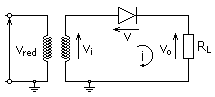
\includegraphics{Circuito_rectificador_media_onda.png}
    \caption{Caption}
    \label{fig:rectificadorMedia}
\end{figure}

\subsection{Tensión rectificada}

\begin{itemize}
    \item  Vo (corriente continua de salida) = Vi ( corriente alterna de entrada) = Vs/2 en el rectificador con diodos.
    \item  Vo = Vi = Vs en el rectificador con puente de Graetz.
\end{itemize}

   

Si consideramos la caída de tensión típica en los diodos en conducción, aproximadamente 0,7V; tendremos que para el caso del rectificador de doble onda la Vo = |Vi| - 1,4V.\citep{circuitoOnda}\\


\begin{figure}[h!]
    \centering
    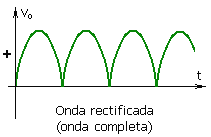
\includegraphics[scale=0.8]{OndaCompleta.png}
   % \caption{Onda Completa}
    \label{fig:my_label}
\end{figure}


\begin{figure}[h!]
    \centering
    \includegraphics[scale=0.5]{Imagenes/rizov.jpg}
    \caption{Gráficas de rizado}
    \label{fig:rizado}
\end{figure}

 
A la forma de onda obtenida en la figura en color rojo se le llama rizado si ahora se mide con un multitester la tensión continua sobre la resistencia de carga se observará que esa medida se aproxima a (Vp-1,4), pero aún no es totalmente continua, la diferencia entre el valor máximo y mínimo del rizado se denomina tensión de rizado pico a pico Vppr y tiene un valor que se puede aproximar con la siguiente fórmula:\citep{FiltroParaCorrienteAlterna}\\

\begin{equation}
    V_{ppr}=\frac{I}{fC}
\end{equation}

Donde I es la corriente continua que se quiere que suministre la fuente de alimentación, f es la frecuencia del rizado que será igual a la frecuencia de la tensión rectificada, que es el doble de la frecuencia del la tensión obtenida en el secundario del transformador que es 50Hz o 60Hz(eso depende del país), por ejemplo si la frecuencia es 50Hz, entonces la frecuencia de rizado será 100Hz; y C es la capacitancia del condensador utilizado como filtro; para que la tensión medida sea totalmente continua, será necesario hacer el rizado lo menor posible esto es  Vppr lo mas pequeño posible.\citep{FiltroParaCorrienteAlterna}\\

Para hacer el Vppr pequeño se tendría que disminuir la corriente, pero en la fuente de alimentación se quiere que este sea lo mayor posible ya que si se disminuye la corriente la fuente no servirá de mucho, otra opción sería aumentar la frecuencia de rizado, pero la frecuencia es una constante 100Hz o 120Hz; otr< opción que queda es que la capacitancia del condensador de filtro sea un valor grande, lo  cual puede ser, pero resulta que la capacitancia no debe tener un valor demasiado grande ya que esto afectaría a los diodos y a la bobina del del secundario del transformador.\citep{FiltroParaCorrienteAlterna}



 
 \section{Material}

\begin{itemize}
    \item Resistencias de 1 [k$\Omega$]
    \item 4 Diodos 1N4001
    \item Transformador de 12 [V] a 1 [A]
    
\end{itemize}

\section{Desarrollo}

\subsection{Circuito Rectificador de media Onda}

Para éste circuito se usó un transformado con tap central de 12 [V] a 1 [A].\\

\begin{figure}[h!]
    \centering
    \begin{circuitikz}
    
        \draw (0,0) node [transformer](T){};
        \draw  (1,0) to[D,v=D](3,0);  
        \draw  (3,0) to[R,l=R](3,-2.1)
        (1,-2.1)--(3,-2.1)
        (3,-2.1)--(4,-2.1)
        (3,0)--(4,0)
        
        ; 
    \end{circuitikz}
    \caption{Rectificador media Onda}
    \label{fig:rectificadorMediaO}
\end{figure}

De la figura \ref{fig:rectificadorMediaO} se colocó en el canal 1 del osciloscopio la salida directa del transformador, y en el canal 2 la salida que da el circuito entre los 2 nodos del resistor.\\

\begin{figure}
    \centering
    
   
\begin{tikzpicture}
\begin{axis}[
    axis lines = left,
    xlabel = $t$,
    ylabel = {$[V]$},
]


%Entrada al circuito

\addplot [
    domain=-(4*3.14159):+(4*3.14159), 
    samples=100, 
    color=blue,
]
{15*sin(deg(x))-30};

%Media Onda
\addplot [
    domain=-(4*3.14159):+(-3*3.14159), 
    samples=100, 
    color=red,
]
{13*sin(deg(x))};

\addplot [
    domain=+(-3*3.14159):(-2*3.14159), 
    samples=100, 
    color=red,
]
{0};
\addplot [
    domain=-(2*3.14159):+(-1*3.14159), 
    samples=100, 
    color=red,
]
{13*sin(deg(x))};

\addplot [
    domain=+(-1*3.14159):(0*3.14159), 
    samples=100, 
    color=red,
]
{0};
\addplot [
    domain=-(0*3.14159):+(1*3.14159), 
    samples=100, 
    color=red,
]
{13*sin(deg(x))};

\addplot [
    domain=+(1*3.14159):(2*3.14159), 
    samples=100, 
    color=red,
]
{0};

\addplot [
    domain=(2*3.14159):+(3*3.14159), 
    samples=100, 
    color=red,
]
{13*sin(deg(x))};

\addplot [
    domain=+(3*3.14159):(4*3.14159), 
    samples=100, 
    color=red,
]
{0};


\addlegendentry{$15 V_{p}$}

    color=blue,
   
 \addlegendentry{$13 V_{p}$}

    color=red,
   
\end{axis}
\end{tikzpicture}

 \caption{Señal circuito rectificador de media onda}
    \label{fig:senalMediaO}
\end{figure}

En la figura \ref{fig:senalMediaO} podemos observar el comportamiento del circuito rectificador de media onda, en él se puede apreciar la señal que entrega el transformador en color azul contra la señal de salida en color rojo.\\


\begin{figure}[h!]
    \centering
    \begin{circuitikz}
    
        \draw (0,0) node [transformer](T){};
        \draw  (1,0) to[D,v=D](3,0);  
        \draw  (3,0) to[R,l=R](3,-2.1)
        (1,-2.1)--(3,-2.1)
        (3,-2.1)--(4,-2.1)
        (3,0)--(4,0)
        
        ; 
    \end{circuitikz}
    \caption{Rectificador media Onda}
    \label{fig:rectificadorMediaO}
\end{figure}

De la figura \ref{fig:rectificadorMediaO} se colocó en el canal 1 del osciloscopio la salida directa del transformador, y en el canal 2 la salida que da el circuito entre los 2 nodos del resistor.\\

\begin{figure}
    \centering
    
   
\begin{tikzpicture}
\begin{axis}[
    axis lines = left,
    xlabel = $t$,
    ylabel = {$[V]$},
]


%Entrada al circuito

\addplot [
    domain=-(4*3.14159):+(4*3.14159), 
    samples=100, 
    color=blue,
]
{15*sin(deg(x))-30};

%Onda Rectificada
\addplot [
    domain=-(4*3.14159):+(-3*3.14159), 
    samples=100, 
    color=red,
]
{13*sin(deg(x))};

\addplot [
    domain=-(3*3.14159):+(-2*3.14159), 
    samples=100, 
    color=red,
]
{-13*sin(deg(x))};

\addplot [
    domain=-(2*3.14159):+(-1*3.14159), 
    samples=100, 
    color=red,
]
{13*sin(deg(x))};

\addplot [
    domain=-(1*3.14159):+(-0*3.14159), 
    samples=100, 
    color=red,
]
{-13*sin(deg(x))};

\addplot [
    domain=-(0*3.14159):+(1*3.14159), 
    samples=100, 
    color=red,
]
{13*sin(deg(x))};

\addplot [
    domain=(1*3.14159):+(2*3.14159), 
    samples=100, 
    color=red,
]
{-13*sin(deg(x))};

\addplot [
    domain=(2*3.14159):+(3*3.14159), 
    samples=100, 
    color=red,
]
{13*sin(deg(x))};

\addplot [
    domain=(3*3.14159):+(4*3.14159), 
    samples=100, 
    color=red,
]
{-13*sin(deg(x))};

\addlegendentry{$15 V_{p}$}

    color=blue,
   
 \addlegendentry{$6.5 V_{p}$}

    color=red,
   
\end{axis}
\end{tikzpicture}

 \caption{Señal circuito rectificador de media onda}
    \label{fig:senalMediaO}
\end{figure}

En la figura \ref{fig:senalMediaO} se puede apreciar la señal de entrada del transformador en color azul, y la señal de salida en rojo rectificada.\\

\section{Discusión}

Logramos comprobar experimentalmente el uso de filtros para la generación de una corriente alterna pulsante a partir de la corriente proporcionada por un transformador, es importante revisar los valores de éstos filtros ya que si sus valores de diseño están al límite o son inferiores a los voltajes suministrados éstos podrían no funcionar adecuadamente o vencerse por un mal funcionamiento.\\

También apreciamos las características del diodo, es decir sus valores de voltaje y de corriente en polarización directa y en inversa, comparándola con la curva del diodo real logramos apreciar que aun estando en polarización inversa el diodo presente corriente entres sus terminales, pero aun así es significativamente menos a la corriente proporcionada se éste se polariza en directa. \\

\section{Conclusión}

Es importante comprender las características del diodo para poderlo incorporar en circuitos de transformación de corriente (AC a DC), y cómo a través de su funcionamiento es posible. Es importante también tener en cuenta la polarización inversa de un diodo, ya que aunque el diodo de propósitos generales no se trabaja con su voltaje de ruptura, sino de funcionamiento, es un concepto importante para el diodo Zener en los próximos experimentos.\\





\bibliographystyle{plain}
\bibliography{Referencias.bib}

\end{document}